\documentclass[12pt,a4paper]{article}
\usepackage{amsmath}
\usepackage{amsfonts}
\usepackage{amsthm}
\usepackage{mathtools}
\newtheorem{theorem}{Theorem}[section]
\newtheorem{definition}{Definition}[section]
\numberwithin{equation}{section}
\usepackage{pgfplots}
\pgfplotsset{width=10cm,compat=1.9}
\graphicspath{ {img/} }
\DeclareGraphicsExtensions{.png,.jpg}

\title{Binary classification}
\author{Kristian Wichmann}

\begin{document}
\maketitle

\section{Basic definitions}
\textit{Binary classification} is a situation where there's two distinct outcomes which we are trying to predict. Associated predictors are known as \textit{binary predictors}.

\subsection{Positives and negatives}
The two outcomes are denoted \textit{positives} and \textit{negatives}, respectively. Given a data point, and the corresponding prediction of a binary predictor, there's four different possibilities:
\begin{itemize}
\item\textit{True positive}: Both the actual outcome and the prediction is positive.
\item\textit{False positive}: The prediction is positive, but the actual outcome is negative. This is also known as a \textit{type I error}. 
\item\textit{False negative}: The prediction is negative, but the actual outcome is positive. This is also known as a \textit{type II error}. 
\item\textit{True negative}: Both the actual outcome and the prediction is negative.
\end{itemize}

\subsection{The confusion matrix}
The frequency of the four above-mentioned events are usually presented in matrix form, in what is known as the \textit{confusion matrix}. It is shown in table \ref{table:confusion_matrix}, where TP means 'True Positive' and so on.

\begin{table}
\centering
\label{table:confusion_matrix}
\begin{tabular}{c|c|c|}
\cline{2-3}
\multicolumn{1}{l|}{Actual/Predicted} & Positive & Negative \\ \hline
\multicolumn{1}{|c|}{Positive}        & TP       & FN       \\ \hline
\multicolumn{1}{|c|}{Negative}        & FP       & TN       \\ \hline
\end{tabular}
\caption{The confusion matrix.}
\end{table}

The entries can either be specified absolutely or relatively.

\section{Sensitivity, specificity and prevalence}
A common way of describing a predictor is through \textit{sensitivity} and \textit{specificity}:
\begin{itemize}
\item Sensitivity - also known as \textit{recall} or \textit{true positive rate} (TPR) - is the rate of actual positives that are classified as such. It can be expressed as:
\begin{equation}
\textrm{TPR}=\frac{\textrm{TP}}{\textrm{TP}+\textrm{FN}}
\end{equation}
\item Specificity - also known as \textit{true negative rate} (TNR) - is the rate of actual negatives that are classified as such. It can be expressed as:
\begin{equation}
\textrm{TNR}=\frac{\textrm{TN}}{\textrm{TN}+\textrm{FP}}
\end{equation}
\end{itemize}

One might think, that if a predictor has a high specificity and sensitivity, then it is useful. It turns out that this is not automatically true: \textit{prevalence}, i.e. the overall occurence rate of positives also plays a role. The prevalence is $\textrm{TP}+\textrm{FN}$.

\subsection{Example}
Assume that a disease has a prevalence of $0.1\%$ in a given population. A screening procedure with a specificity of $99\%$ and a sensitivity of $95\%$. At first glance, this looks like a good predictor. But in practice, it is less impressive:

Since only $0.1\%=0.001$ of the population actually has the disease (positive), $99.9\%$ has not (negative). Of that $0.1\%$, $99\%$ are true positives:
\begin{equation}
\textrm{TP}=0.001\cdot 0.99=0.00099
\end{equation}
The final $1\%$ of the actual positives are false negatives:
\begin{equation}
\textrm{TP}=0.001\cdot 0.01=0.00001
\end{equation}
Out of the actual positives, $95\%$ are true negatives:
\begin{equation}
\textrm{TN}=0.999\cdot 0.95=0.94905
\end{equation}
The $5\%$ of the actual negatives are false positives:
\begin{equation}
\textrm{FP}=0.999\cdot 0.05=0.04995
\end{equation}
The corresponding confusion matrix is shown in table \ref{table:example_confusion_matrix}.

\begin{table}
\centering
\label{table:example_confusion_matrix}
\begin{tabular}{c|c|c|}
\cline{2-3}
\multicolumn{1}{l|}{Actual/Predicted} & Positive & Negative \\ \hline
\multicolumn{1}{|c|}{Positive}        & 0.00099  & 0.00001  \\ \hline
\multicolumn{1}{|c|}{Negative}        & 0.04995  & 0.94905  \\ \hline
\end{tabular}
\caption{Example confusion matrix.}
\end{table}

\section{Positive and negative predictive value}
In practice, the following statistics are often of great importance:
\begin{itemize}
\item The \textit{positive predictive value} (PPV) is the conditional probability that a sample is actually positive given that the prediction is positive. It can be expressed:
\begin{equation}
\textrm{PPV}=\frac{\textrm{TP}}{\textrm{TP}+\textrm{FP}}
\end{equation}
\item The \textit{negative predictive value} (NPV) is the conditional probability that a sample is actually negative given that the prediction is negative. It can be expressed:
\begin{equation}
\textrm{NPV}=\frac{\textrm{TN}}{\textrm{TN}+\textrm{FN}}
\end{equation}
\end{itemize}

\subsection{Example}
In the example above, the positive predictive value is:
\begin{equation}
\textrm{PPV}=\frac{0.00099}{0.00099+0.04995}\approx 0.019
\end{equation}
The negative predictive value is:
\begin{equation}
\textrm{NPV}=\frac{0.94905}{0.94905+0.00001}\approx 1.000
\end{equation}
So, the screening is very good at actually predicting negatives: If the test is negative, you're almost certain not to have the disease. However, if the test is positive, there's only a $1.9\%$ chance that you actually have the disease! This is not very reassuring! The deeper reason for this low number, is that since the prevalence is low, there ends up being a comparatively large number of false positives, even if the specificity is high.

\begin{figure}
\centering
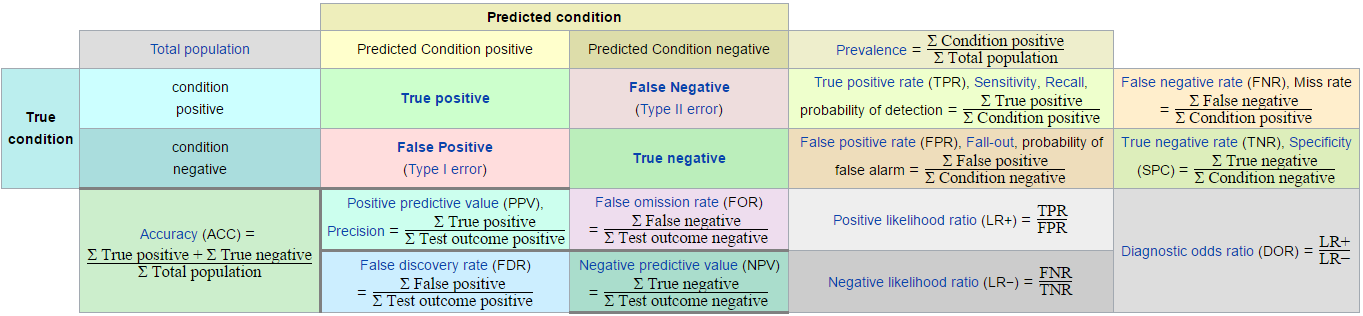
\includegraphics[width=\textwidth]{confusion_matrix_extended}
\caption{Confusion matrix and derived statistics. Source: Wikipedia.}
\label{fig:confusion_matrix_extended}
\end{figure}

\end{document}